\chapter{Joint Inversion}\label{Chp:cook:joint inversion}


A striking interpretation of a joint inversion 3D model of gravity and magnetic data could solve a big problem of exploration geophysics. Traditionally inversion of magnetic and gravity data provide a 3D physical rock property model separately. However the inversion different type of datasets could supplement the result. In the meantime joint inversion by making more contrants on characteristics modify the outcome.

In this section a new package is significantly presented to provide a joint model of density and magnetic susceptibility which undertake an apparent discrepancy in terms of geolophysical approach. This package is based on geological smooth model in density and magnetic susceptibility variations.



\section{Input File} 

According to the escript which is configured a prominent joint inversion in gravity and magnetic data, input data have contains gravity and magnetic anomalies data sets. In previous sections, gravity and magnetic data and their corrections, which need to invert, were distinguished in detail.

However it does not need to have data in one input file. They could be seperatly but it have to be mentioned that the inversion just run in the overlaping area with properly result.

Also its speacing is not important though the finer spacing , the better result. and its spacing could be differ in meter. 

Ferthermore the script file for 2D and 3D inversion in apart and it have to be selected to have 2d or 3D inversion.

A small part of sample of inversion_gravmag_3d:

\begin{verbatim}
depth_offset = 10. * U.km
n_humps_h = 3
n_humps_v = 1
n_humpsm_h =2
n_humpsm_v =1
mu = 100.
n_cells_in_data = 30
latitude = -28.5
l_data = 100. * U.km
l_pad = 40. * U.km
THICKNESS = 20. * U.km
l_air = 6. * U.km
\end{verbatim}

inversion_gravmag file consist many options to implement which control how joint inversion is performed such as padding area, depth , MU factor,\ldots. which in previous section was explaind in deatails. just some items are fixed for joint inversion such as mu.


\begin{description} 	
\item[latitude]this is refered to the area of gathering data sets to calculate the main reference magnetic field. which is selected -28 for east Australia.


\item[mu]It is defined in accordance with the noise of data it is 100 for this section.

\end{description}

\section{Output File}

After preparing input files and submitting the escript to run inversion, an output file will be created to show result of inversion. This file has silo extension and contain both density and susceptibility. Moreover it display those values separately in a 2D or 3D model. The inversions dimention is related to our dessicion at the time of start up.

\section{Reference}

This is a 3D model as an example with three different density humps and two different susceptibility humps in horizon which have nine density humps and four susceptibility humps. Two first images show the reference synthetic datasets (\ref{fig:joint3D4mag6grav-gref} and \ref{fig:joint3D4mag6grav-mref}) and two last images indicate result after joint inversion in two both magnetic and gravity.(\ref{fig:joint3D4mag6grav-g} and \ref{fig:joint3D4mag6grav-m})
 
\begin{verbatim}
n_humps_h = 3
n_humps_v = 1
n_humpsm_h =2
n_humpsm_v =1
mu=100
\end{verbatim}

\begin{figure}
\centering
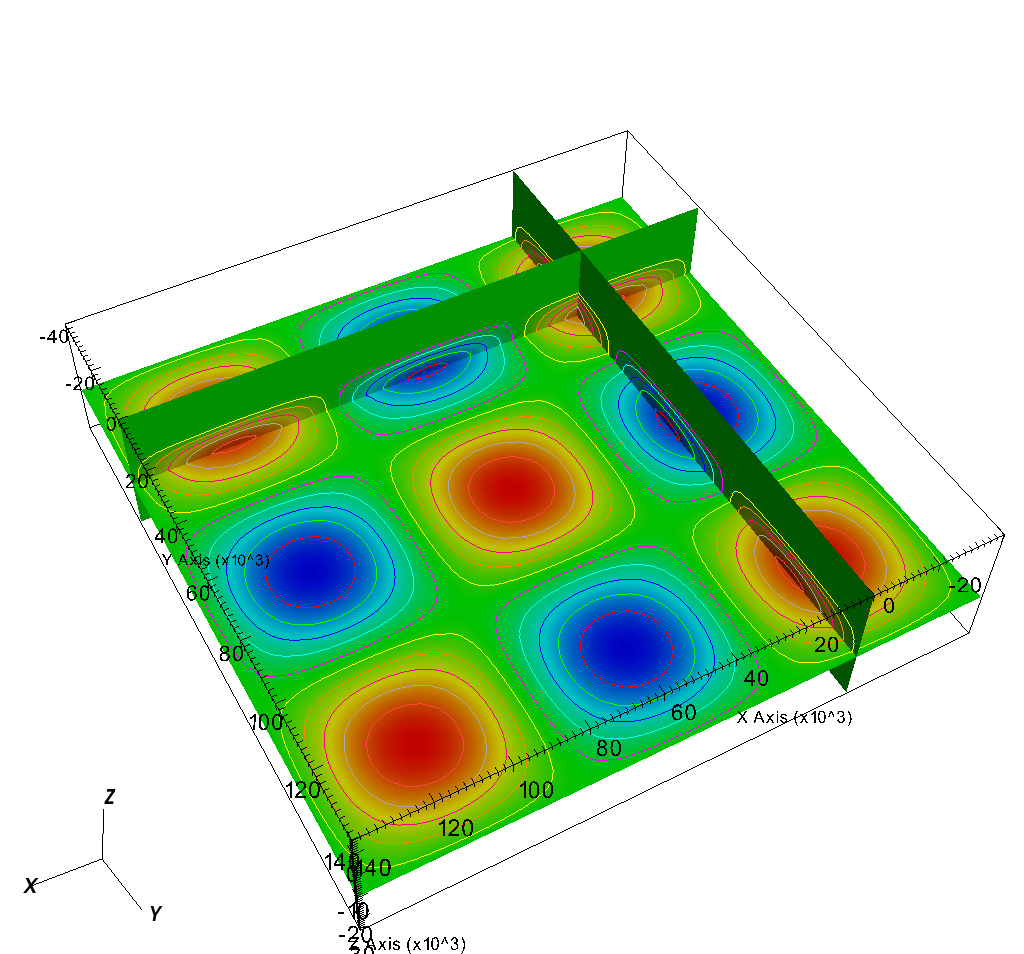
\includegraphics[width=\textwidth]{joint3D4mag6grav-gref.png}
\caption{3D reference density model}
\label{fig:joint3D4mag6grav-gref}
\end{figure}


\begin{figure}
\centering
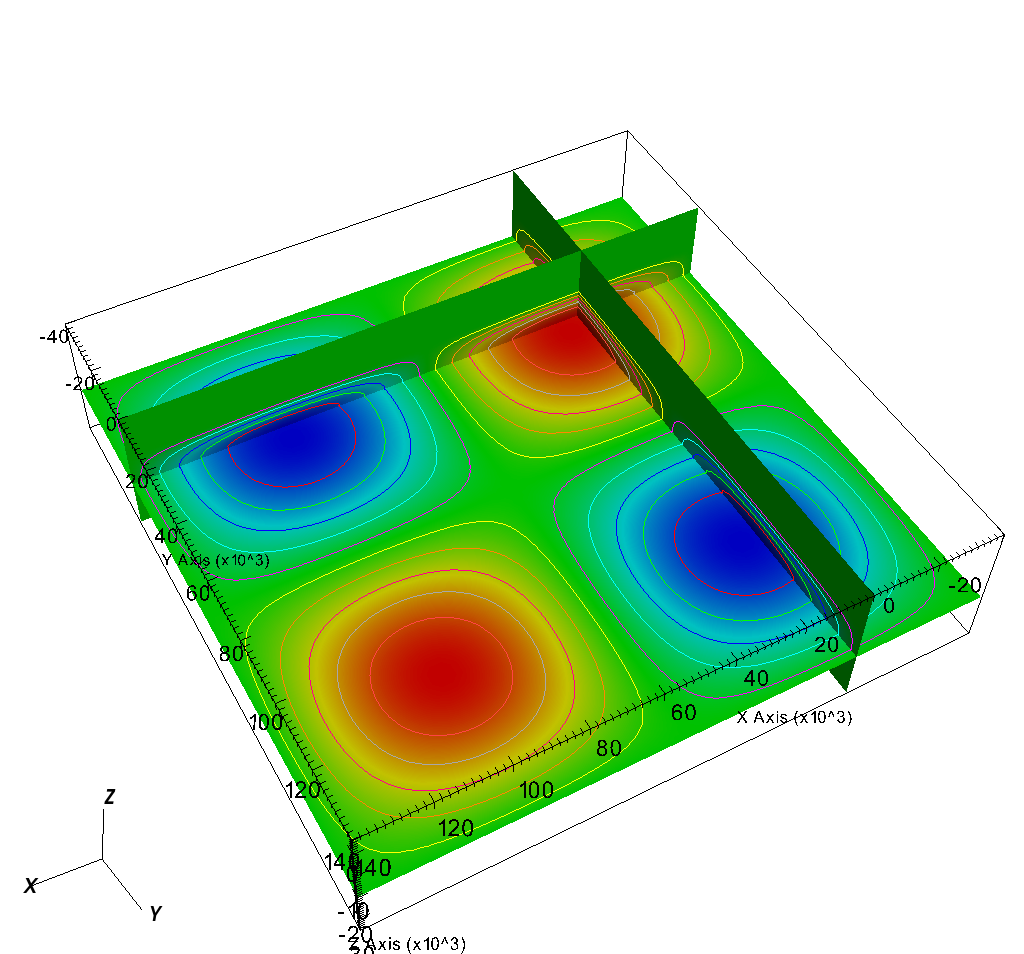
\includegraphics[width=\textwidth]{joint3D4mag6grav-mref.png}
\caption{3D reference susceptibility model}
\label{fig:joint3D4mag6grav-mref}
\end{figure}


\begin{figure}
\centering
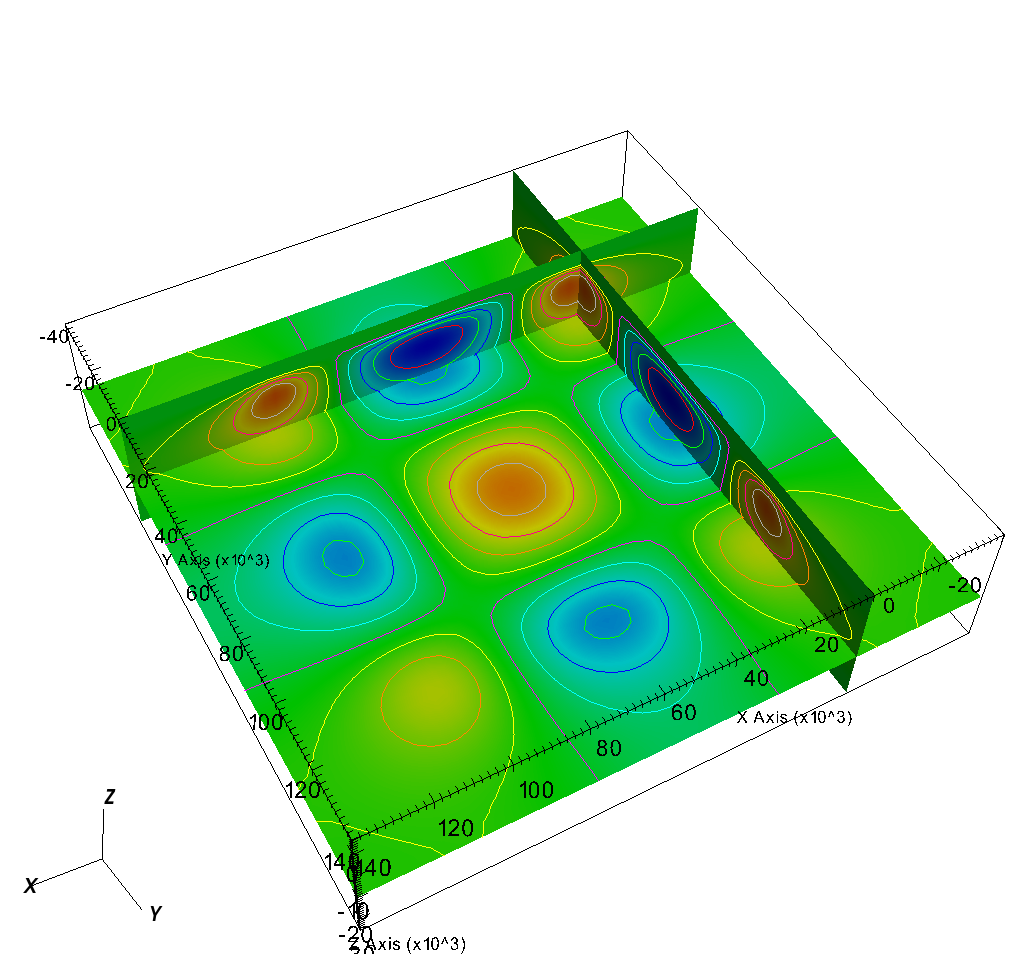
\includegraphics[width=\textwidth]{joint3D4mag6grav-g.png}
\caption{3D result density model}
\label{fig:joint3D4mag6grav-g}
\end{figure}


\begin{figure}
\centering
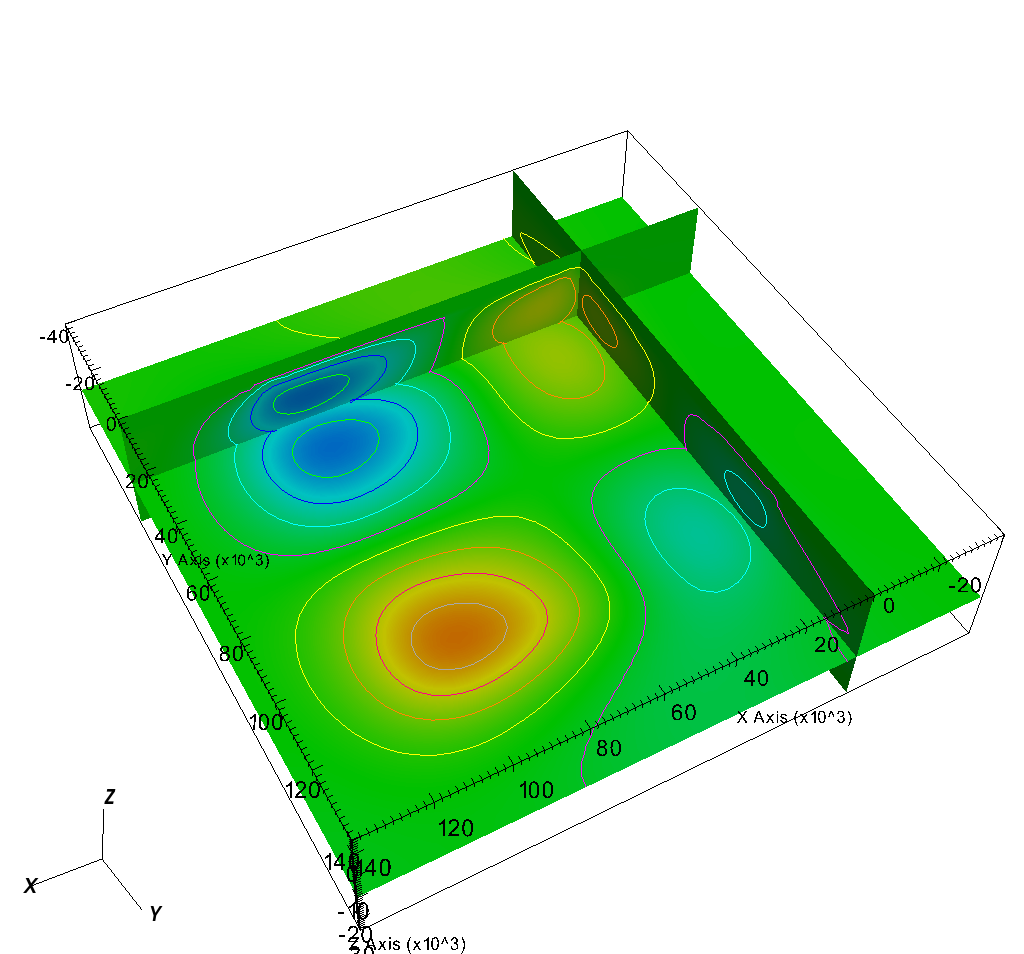
\includegraphics[width=\textwidth]{joint3D4mag6grav-m.png}
\caption{3D result magnetic model}
\label{fig:joint3D4mag6grav-m}
\end{figure}

